\documentclass[10pt,a4paper]{article}
\usepackage[T1]{fontenc}
\usepackage[utf8]{inputenc}
\usepackage{lmodern}
\usepackage[margin=25mm]{geometry}
\usepackage{amsmath,amssymb,booktabs,graphicx}
\usepackage{caption,float,needspace}
\usepackage[hidelinks]{hyperref}
\captionsetup{font=small}
\setlength{\parindent}{0pt}
\setlength{\parskip}{5pt}
\setlength{\emergencystretch}{2em}
\newcommand{\ind}{\mathbf{1}}
\hypersetup{pdftitle={Bootstrap uncertainty in sidewalk-hazard rankings}}
\begin{document}
\section*{Bootstrap uncertainty in sidewalk-hazard rankings}

We study whether uncertainty across repeated classifier fits improves the ordering
of sidewalk images for hazard review. The analysis concerns only the binary
hazard task, with a fixed review budget of 46 images. We compare three approaches:
penalizing probability uncertainty, summarizing rank distributions, and deriving
a consensus from pairwise outranking probabilities. Two reference rankings are
retained: the previously selected single DINO hazard head and the unadjusted mean
of the bootstrap heads.

\section{Training independent heads with bootstrapping}
\label{sec:training}
The ensemble uses the previously selected Pittsburgh-only configuration. A frozen
DINOv3 ViT-B/16 backbone maps each RGB $224\times224$ image, with ImageNet
normalization, to a 768-dimensional CLS feature vector $z_i$. We train $B=128$
separate linear hazard heads, each producing
\begin{equation}
p_i^{(b)}=\operatorname{sigmoid}\!\left(w_b^{\mathsf T}z_i+c_b\right),
\qquad b=1,\ldots,B.
\end{equation}
The backbone is shared and remains fixed. Other-city training images are not used.

The training set has 1,276 records: 527 hazards and 749 non-hazards. To keep exact
image duplicates together, records are grouped by their RGB pixel hash. This
gives 1,236 groups, including 40 duplicate pairs. Groups are stratified by their
binary-label composition: the numbers of hazard and non-hazard records in each
group. For each head and each stratum, we sample the original number of groups
\emph{with replacement}, include all records from each sampled group, and shuffle
the resulting records. Thus every head receives 1,276 draws with the original
class counts, while the sampled records and their multiplicities vary. The
samples contain 784--840 distinct records, with a mean of 807.3.

Each head has separate bootstrap, parameter-initialization and minibatch-shuffle
random seeds. All heads use Adam with learning rate $3\times10^{-5}$, weight decay
$0.01$, batch size 64 and 5,000 parameter updates, minimizing unweighted binary
cross-entropy. We retain the final checkpoint of every head; there is no
validation-based early stopping or selection among the 128 members. Training
updates use only the training split. This yields 128 aligned hazard probabilities
per observation: column $b$ always refers to the same head for every image.

The original reference model is the single non-bootstrap hazard head retained
from the earlier validation-based model selection. It was trained on the full
Pittsburgh training split, using the same selected configuration. Its predictions
are used directly; its score is not the average validation score over the original
configuration's multiple training seeds. The second reference averages the 128
bootstrap predictions. Evaluation uses the same images and labels for all methods.

\section{Uncertainty-adjusted probability ranking}
\label{sec:adjusted}
For observation $i$, define the ensemble mean and sample standard deviation
\begin{equation}
\mu_i=\frac{1}{B}\sum_{b=1}^{B}p_i^{(b)},\qquad
s_i=\sqrt{\frac{1}{B-1}\sum_{b=1}^{B}\left(p_i^{(b)}-\mu_i\right)^2}.
\end{equation}
The unadjusted ensemble ranking orders images by decreasing $\mu_i$. To favor
predictions that are stable across fitted heads, the uncertainty-adjusted score is
\begin{equation}
S_i(\lambda)=\mu_i-\lambda s_i.
\end{equation}
Here $s_i$ is variability across heads, not the standard error of the ensemble
mean. Scores are not clipped to $[0,1]$. Exact score ties use ascending sample ID.

We tune $\lambda$ on validation precision@46 over the fixed grid
$\{0,0.05,\ldots,4\}$, choosing the smallest value among tied maxima. A fixed fifth
percentile of the 128 probabilities is a second conservative comparator; its
quantile is not tuned. Both methods favor low-uncertainty predictions, but neither
is guaranteed to maximize the number of true hazards retrieved. If the mean
probabilities equal the relevant predictive expectations, choosing the largest
means maximizes expected hazard yield at a fixed budget. The SD penalty instead
introduces an additional preference for stability.

\section{Rank distributions and selection frequencies}
\label{sec:ranks}
Rather than penalize probabilities, we can measure uncertainty in an observation's
position. For each head, all observations are ranked together by decreasing
hazard probability, with rank 1 the highest and exact score ties assigned
midranks. Let $r_i^{(b)}$ denote this rank. We report
\begin{equation}
\overline r_i=\frac{1}{B}\sum_b r_i^{(b)},\qquad
I_i=\left[Q_{0.025}(r_i^{(1:B)}),Q_{0.975}(r_i^{(1:B)})\right],
\end{equation}
where empirical quantiles use linear interpolation. The interval describes
midrank variation across refits, without adding random tie-breaking noise.

We also report the frequency of ranking first and of appearing in the top $k$.
For head $b$, let $a_i^{(b)}$ count observations with strictly larger scores and
$t_i^{(b)}$ count observations tied with $i$, including $i$ itself. Allocating tied
slots equally gives
\begin{equation}
\widehat P_k(i)=\frac{1}{B}\sum_b
\min\!\left\{1,\max\!\left\{0,\frac{k-a_i^{(b)}}{t_i^{(b)}}\right\}\right\}.
\end{equation}
We use $k=1$ and $k=46$; these frequencies sum over observations to 1 and 46,
respectively. They describe selection stability, not the chance that an image
is a true hazard.

Two fixed orderings are compared: increasing expected rank $\overline r_i$ and
decreasing top-46 frequency $\widehat P_{46}(i)$. Expected-rank ties use sample ID;
frequency ties use expected rank, then sample ID. No hazard labels determine
either ordering. The expected-rank ordering is weighted Borda aggregation, as
made explicit by the pairwise identity in the next section.

\section{Pairwise outranking and consensus}
\label{sec:pairwise}
For every pair of observations, compare predictions from the \emph{same} head:
\begin{equation}
W_{ij}=\frac{1}{B}\sum_b\ind[p_i^{(b)}>p_j^{(b)}],\qquad
T_{ij}=\frac{1}{B}\sum_b\ind[p_i^{(b)}=p_j^{(b)}].
\end{equation}
This preserves dependence between predictions. The strict outranking and tie
frequencies satisfy $W_{ij}+W_{ji}+T_{ij}=1$, with $W_{ii}=0$ and $T_{ii}=1$.
If two observations tie in every head, both strict probabilities are zero;
this does not mean that each image is ranked below the other. Full matrices
retain image identifiers, and heatmaps show $W_{ij}$ with the same ordering on
both axes. Pairwise probabilities also connect the analyses through
\begin{equation}
\overline r_i=1+\sum_{j\ne i}\left(W_{ji}+\tfrac12T_{ij}\right).
\end{equation}

A pairwise consensus instead seeks a permutation that maximizes agreement with
all heads' pairwise orderings. Writing $C_{ij}=BW_{ij}$, the Kemeny objective is
\begin{equation}
\pi^*\in\operatorname*{arg\,max}_{\pi}
\sum_{1\leq a<b\leq N}C_{\pi(a),\pi(b)}.
\label{eq:objective}
\end{equation}
Giving half-credit to score ties adds the same constant for every permutation,
so it does not change the optimum. This objective differs from both expected
rank and true-hazard yield in the first 46 positions.

Majority preferences may form cycles. We first decompose the majority graph into
strongly connected components, including edges in both directions for equal
pairwise preferences. Cross-component preferences then have an acyclic ordering.
Within each component, Borda ordering and improving insertions provide a feasible
solution. A binary linear-ordering program uses $x_{ij}=1$ when $i$ precedes $j$
for $i<j$, and the transitivity constraints
\begin{equation}
0\leq x_{ij}+x_{jk}-x_{ik}\leq1,\qquad i<j<k.
\end{equation}
Violated triangle constraints are added iteratively. A feasible permutation and
a relaxation bound are maintained: matching the bound, or an integer objective
gap strictly below one, certifies optimality. The optimizer receives probabilities
only, without true hazard labels. Numerical certificates are reported with the
results below.

\section{Results}
\label{sec:results}
\subsection{Validation comparison}
We rank all 382 validation images, of which 157 are hazards, using a fixed budget
$k=46$ (12.04\% of the split). For ordering $\pi$ and hazard indicator $y_i$, define
\begin{equation}
\operatorname{Precision@46}=\frac{\sum_{a=1}^{46}y_{\pi(a)}}{46},\qquad
\operatorname{Recall@46}=\frac{\sum_{a=1}^{46}y_{\pi(a)}}{\sum_i y_i}.
\end{equation}
All images are eligible for ranking; no binary probability threshold is applied.
The primary comparison is precision@46. With a fixed split and review budget,
recall@46 contains the same ordering information and cannot break a precision tie.

The SD-penalty sweep attains its maximum at eight grid values, $\lambda=0$ through
$0.35$, each retrieving 34 hazards. All other searched values retrieve 33. The
smallest-maximizer rule selects $\lambda=0$, making the adjusted ranking identical
to the unadjusted ensemble mean. The lower-quantile comparator retrieves 32.
The original single head, mean, expected rank, top-46 frequency and pairwise
consensus each retrieve 34 validation hazards (Table~\ref{tab:validation}).
\begin{table}[H]
\centering
\caption{Validation comparison on 382 images, including 157 hazards. Precision and recall are percentages. $^{\dagger}$The original model is selected by the parsimony tie-break described below.}
\label{tab:validation}
\small
\begin{tabular}{lrrr}
\toprule
Ranking & Hazards & Precision@46 & Recall@46 \\
\midrule
Original single head (no bootstrap)$^{\dagger}$ & 34/46 & 73.91 & 21.66 \\
Unadjusted mean (128 heads) & 34/46 & 73.91 & 21.66 \\
Mean minus SD penalty ($\lambda=0$) & 34/46 & 73.91 & 21.66 \\
Fifth probability percentile & 32/46 & 69.57 & 20.38 \\
Expected rank (Borda) & 34/46 & 73.91 & 21.66 \\
Top-46 selection frequency & 34/46 & 73.91 & 21.66 \\
Pairwise consensus (Kemeny) & 34/46 & 73.91 & 21.66 \\
\bottomrule
\end{tabular}
\end{table}
\begin{figure}[H]
\centering
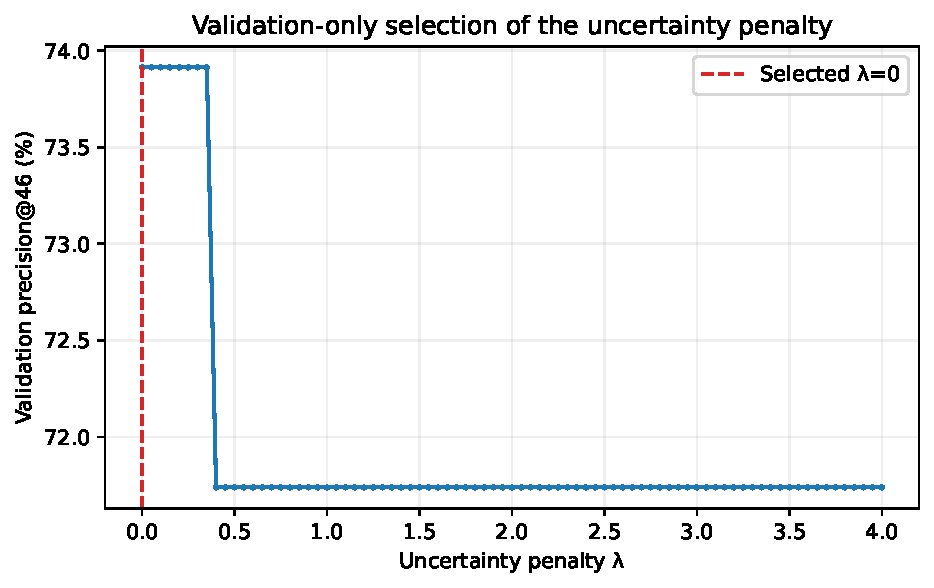
\includegraphics[width=.76\linewidth]{figures/point_2_validation_lambda_sweep.pdf}
\caption{Validation-only tuning of the SD penalty. The smallest maximizing value is $\lambda=0$; no test scores enter this sweep.}
\label{fig:lambda}
\end{figure}

\Needspace{14\baselineskip}
\subsection{Selection between the two reference rankings}
\label{sec:selection}
The original single head and the unadjusted 128-head mean are tied at
$34/46=73.91\%$ validation precision, and no uncertainty-aware comparator exceeds
this result. Validation therefore provides no strict performance winner between
the two reference rankings. We resolve the tie by parsimony: retain the already
selected model that requires only one head rather than 128.

\textbf{We select the original single DINO head without bootstrapping.}
This is a simplicity tie-break among validation-equivalent candidates, not evidence
that the original model is more accurate. The ensemble mean is equally supported
by this validation metric. The lower-quantile ranking is worse on validation;
the remaining approaches offer no validation precision advantage to justify
replacing the reference model. The following test results are reported after this
choice and do not change it.

\subsection{Test performance after selection}
\label{sec:test}
The test split contains 380 images, including 174 hazards. The same budget of 46
images corresponds to 12.11\% of this split. Table~\ref{tab:test} evaluates all
rankings with the methods and SD penalty fixed by the preceding analysis.
\begin{table}[H]
\centering
\caption{Test comparison after the validation-based selection, on 380 images including 174 hazards. $^{\dagger}$Previously selected original model; the selection is not changed using this table.}
\label{tab:test}
\small
\begin{tabular}{lrrr}
\toprule
Ranking & Hazards & Precision@46 & Recall@46 \\
\midrule
Original single head (no bootstrap)$^{\dagger}$ & 26/46 & 56.52 & 14.94 \\
Unadjusted mean (128 heads) & 27/46 & 58.70 & 15.52 \\
Mean minus SD penalty ($\lambda=0$) & 27/46 & 58.70 & 15.52 \\
Fifth probability percentile & 26/46 & 56.52 & 14.94 \\
Expected rank (Borda) & 27/46 & 58.70 & 15.52 \\
Top-46 selection frequency & 28/46 & 60.87 & 16.09 \\
Pairwise consensus (Kemeny) & 27/46 & 58.70 & 15.52 \\
\bottomrule
\end{tabular}
\end{table}

The selected original model retrieves 26 test hazards (56.52\% precision@46).
The unadjusted mean, selected SD-penalty score, expected rank and pairwise
consensus each retrieve 27 (58.70\%). Top-46 frequency retrieves 28 (60.87\%),
while the fifth-percentile score retrieves 26. The ensemble mean therefore has a
one-image test advantage over the selected original model, and frequency ranking
has a two-image advantage. These descriptive differences do not alter the
validation-based choice. One extra hazard changes precision@46 by 2.17 percentage
points; the observed test differences alone do not establish general superiority
or statistical significance.

\subsection{What the uncertainty analyses reveal}
Equal retrieval counts do not imply equally certain image positions.
Table~\ref{tab:stability} summarizes the rank intervals and selection frequencies.
Mean and expected-rank orderings select exactly the same 46 images on each split,
yet the typical rank interval spans many positions. Only 14 images in each split
appear in the top 46 in at least 95\% of heads. Of those stable selections, five
validation images and six test images are labelled non-hazards: stability across
refits can coexist with confident false-positive selections.
\begin{table}[H]
\centering
\caption{Rank stability across 128 heads. Interval widths are in rank positions; other quantities are counts of images.}
\label{tab:stability}
\small
\begin{tabular}{lrr}
\toprule
Statistic & Validation & Test \\
\midrule
Median rank-interval width & 156.2 & 162.2 \\
90th-percentile interval width & 208.4 & 215.8 \\
Intervals crossing rank 46 & 100 & 112 \\
Images with $\widehat P_{46}\geq0.95$ & 14 & 14 \\
Hazards among these stable selections & 9 & 8 \\
Non-hazards among these stable selections & 5 & 6 \\
Images with $\widehat P_{46}>0$ & 158 & 171 \\
\bottomrule
\end{tabular}
\end{table}

The pairwise consensus reaches a certified optimum on both splits
(Table~\ref{tab:optimality}). Relative to expected-rank ordering, it changes 277
validation positions and 279 test positions, but the top-46 sets overlap in 46
and 45 images, respectively. It improves pairwise agreement without changing
the retrieved hazard count. An optimal consensus thus need not improve the
review objective: it weights all image pairs, whereas precision@46 depends
only on which images cross the selection boundary.
\begin{table}[H]
\centering
\caption{Pairwise optimization certificates. Objectives count head-pair agreements, not true hazards.}
\label{tab:optimality}
\small
\begin{tabular}{lrrrr}
\toprule
Split & Feasible objective & Upper bound & Gap & Optimal \\
\midrule
Validation & 8,235,639 & 8,235,639 & 0 & Yes \\
Test & 8,102,338 & 8,102,338 & 0 & Yes \\
\bottomrule
\end{tabular}
\end{table}

The heads are independently fitted conditional on a shared dataset and frozen
representation; their predictions need not be independent. Their intervals and
frequencies capture variation under these bootstrap refits, not all sources of
uncertainty or automatically calibrated posterior probabilities. The validation
set has also supported earlier model selection and the present penalty choice,
so its optimum should not be interpreted as an unbiased population estimate.
Original evaluation observations are retained: validation has 18 duplicate pixel
groups, six with conflicting hazard labels; test has 12 groups, two with
conflicting labels. Such conflicts and shared model errors can persist even
when all heads agree.

The practical finding is that uncertainty summaries expose unstable placements
and comparisons, but none of the tested uncertainty-aware rankings improves
validation precision@46 over the original model or the unadjusted mean. The
single original head remains the selected ranking by the stated parsimony rule;
the ensemble remains useful for reporting rank intervals, selection frequencies
and pairwise comparisons alongside that decision.

\clearpage
\subsection{Rank intervals and pairwise heatmaps}
\begin{figure}[H]
\centering
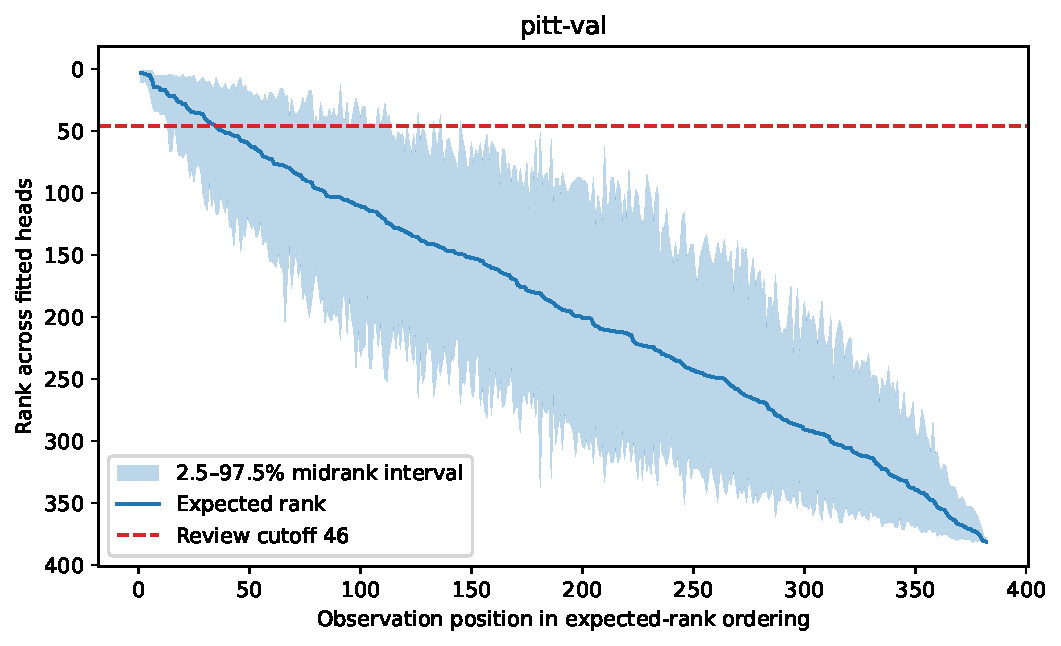
\includegraphics[width=.88\linewidth]{figures/point_3_pitt-val_rank_intervals.pdf}
\caption{Validation rank intervals. Images are ordered by expected rank; shading is the 2.5th--97.5th percentile interval and the dashed line marks rank 46.}
\label{fig:val-intervals}
\end{figure}
\begin{figure}[H]
\centering
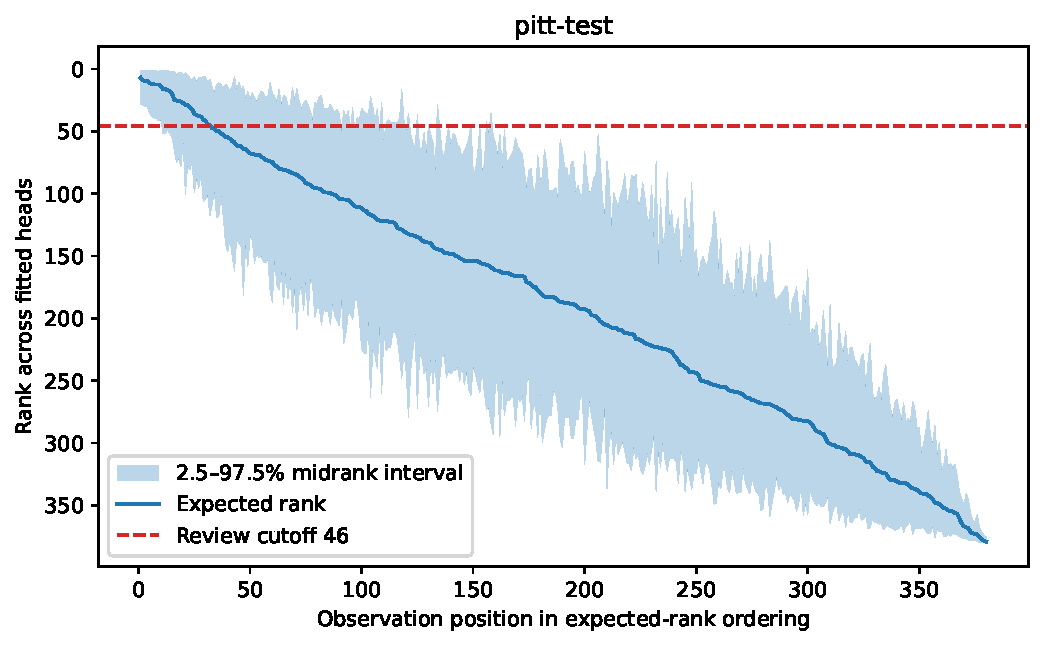
\includegraphics[width=.88\linewidth]{figures/point_3_pitt-test_rank_intervals.pdf}
\caption{Test rank intervals, reported after the selection. Lower ranks indicate higher review priority.}
\label{fig:test-intervals}
\end{figure}
\clearpage
\begin{figure}[H]
\centering
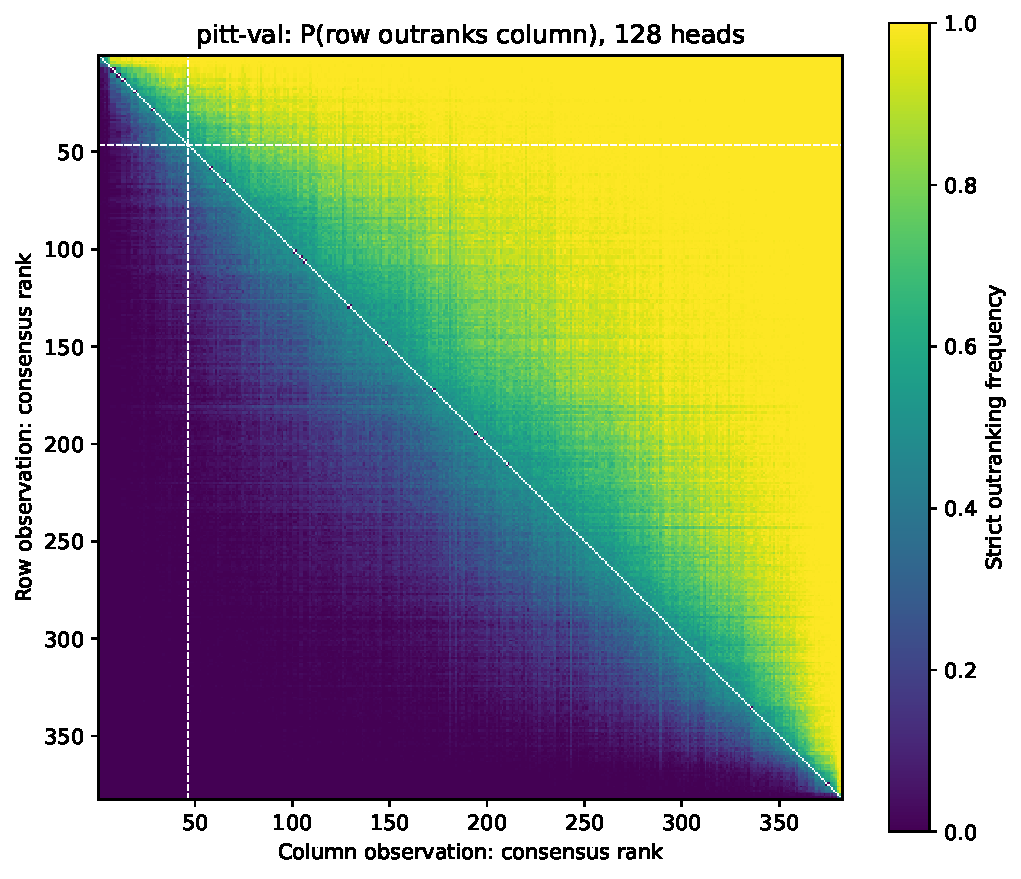
\includegraphics[width=.68\linewidth]{figures/point_4_pitt-val_pairwise_heatmap.pdf}
\caption{Validation strict outranking frequencies $W_{ij}$ in consensus order. A cell is the fraction of heads in which its row image outranks its column image; dashed lines mark the top-46 boundary.}
\label{fig:val-heatmap}
\end{figure}
\begin{figure}[H]
\centering
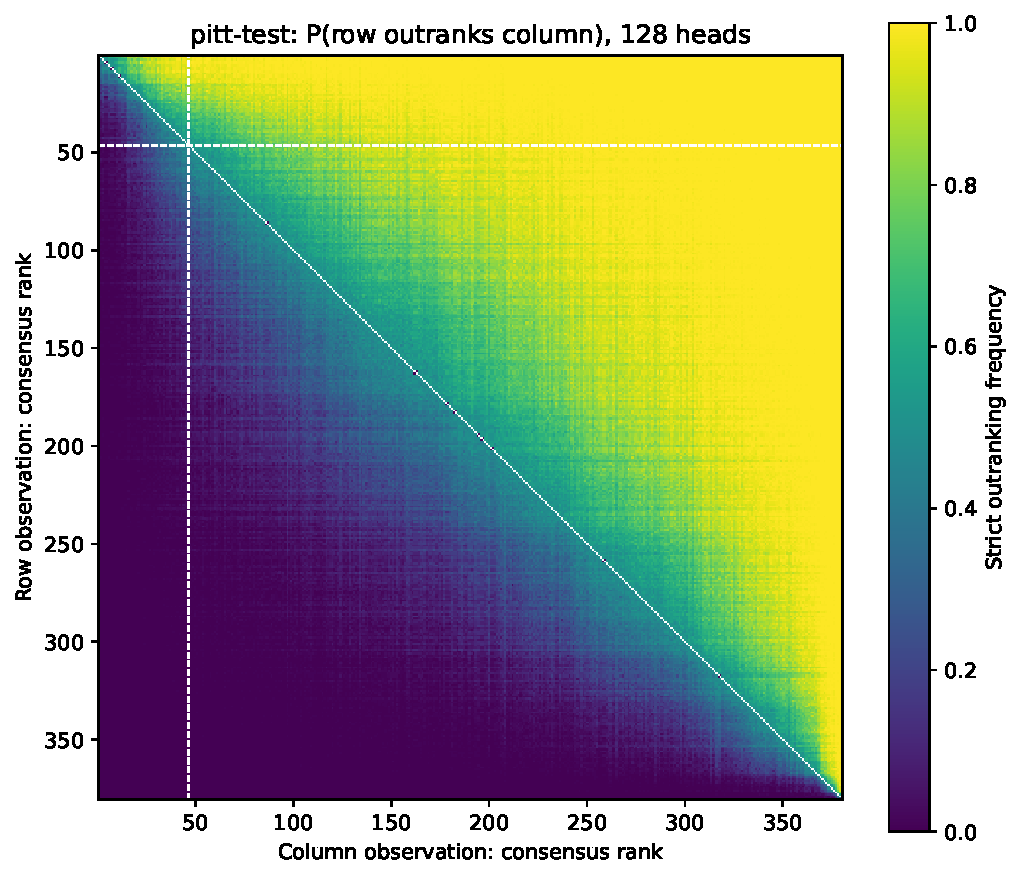
\includegraphics[width=.68\linewidth]{figures/point_4_pitt-test_pairwise_heatmap.pdf}
\caption{Test strict outranking frequencies, reported after selection, on the same $[0,1]$ scale. The diagonal is masked. Exact score ties are represented separately and are not forced to probability 0.5 in this matrix.}
\label{fig:test-heatmap}
\end{figure}
\end{document}
